% Chapter 3
\chapter{分割不含孔洞的凹多边形}


\section{确定多边形方向}
为了便于后续计算,我们规定多边形S的点依次逆时针排列。在计算时我们需要将初始的多边形端点标准化为按逆时针排序。
利用向量叉积的原理,我们可以计算出多边形的方向。
对于多边形的每条边,计算坐标原点到起点的向量,与边起点到终点的向量叉乘并除以2。将结果求和后该向量的模即为多边形面积,而向量z轴方向则代表了多边形的旋转方向。

\begin{equation}
\sum\limits_{i=0}^{n}{\frac{N_i\times (N_{(i+1)\bmod n}-N_i)}{2}}
\end{equation}

计算出初始多边形旋转方向后,即可根据需求调整端点的顺序以标准化多边形的方向。

\section{确认多边形凹凸性}
首先我们遍历多边形的所有内角,检测其是否为凸多边形。

若多边形为凸多边形,转至第二章,直接生成其Delaunay三角划分;若多边形为凹多边形,则采用下面的算法将其分割为数个凸多边形。
\section{确定分割方案}
在这一步我们采用启发式搜索的方式进行分割。

我们定义合法的切割边\(( V_i,V_j) \)满足以下条件:

\begin{itemize}
    \item \(V_i,V_j\)属于同一个多边形
    \item 以\(V_i,V_j\)为端点的线段除端点外与多边形无共同点
    \item \(V_i,V_j\)两个顶点对应的多边形内角至少有一个大于180°
    \item \(0\le i<j\le n-1\)
\end{itemize}
对于原多边形S中的一条合法的切割边,我们采用如下方式来评估其价值:

\begin{itemize}
    \item 设按此方式切割后产生的两个多边形为

    \(S_1:\{ V_0,V_1,\cdots,V_{i-1},V_i,V_j,V_{j+1},\cdots,V_{n-1}\} \)

    \(S_2:\{ V_i,V_{i+1},\cdots,V_{j-1},V_j\}\)

    定义\(C(S_i)\)为多边形\(S_i\)的周长,\quad \(L(V_i,V_j)\)为点\(V_i,V_j\)之间的距离

    \item 定义切割边的基础评分为
    \begin{equation}
        \frac {\min(C(S_1),C(S_2))}{L(V_i,V_j)}
    \end{equation}
    \item 定义切割边的评分修正为
    \begin{equation}
        \frac {\min(\angle V_jV_iV_{i-1},\angle V_jV_iV_{i+1},\angle V_iV_jV_{j-1},\angle V_iV_jV_{j+1})}{90^\circ}
    \end{equation}

    若切割边两个端点对应的内角均>180°则评分修正额外*10

    \item 每条边的价值最终评估为基础评分*评分修正。
    
\end{itemize}

遍历多边形,对于每一个内角大于180°的顶点,采用此算法\upcite{金文华1999简单多边形可见点问题的快速求解算法}快速求出以该点为端点的所有合法切割边,计算其价值并加入记录。

\begin{figure}[htp]
    \centering
    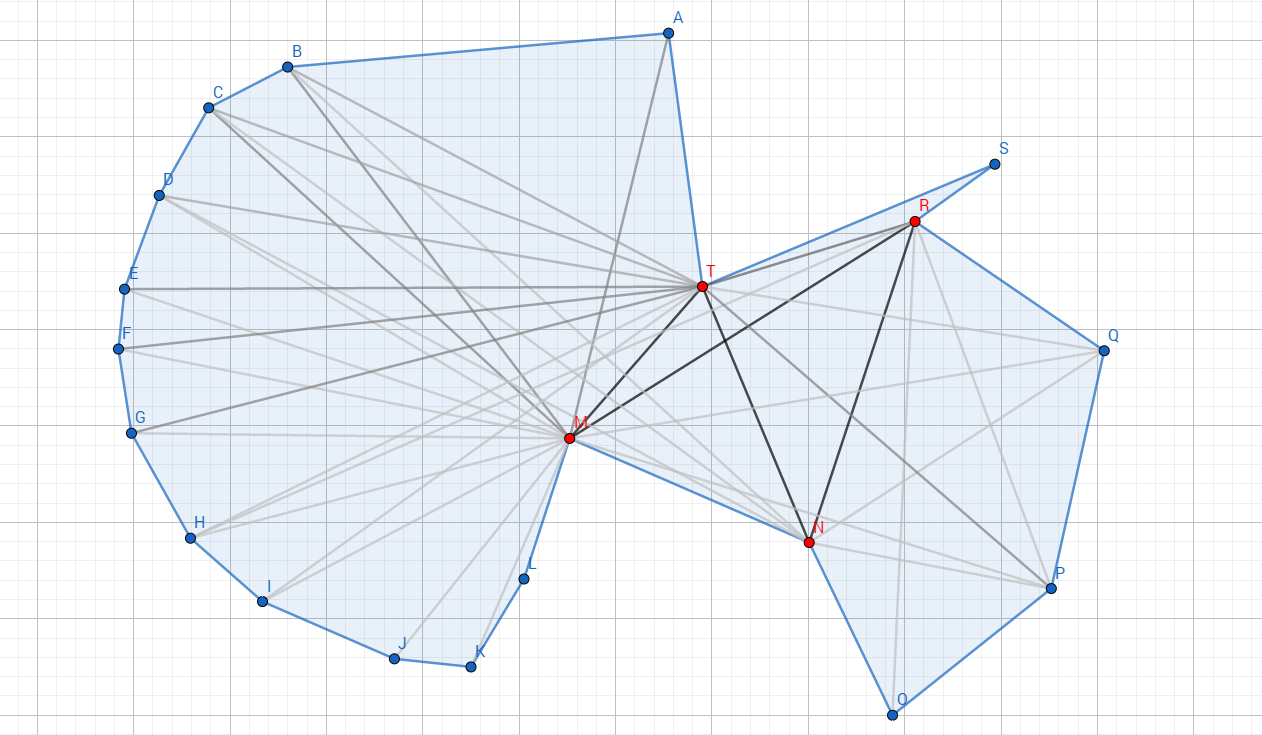
\includegraphics[width=0.5\textwidth]
    {figures/pass1.png}
    \caption{对候选边进行估价}
    \label{pass1}
\end{figure}

接下来对于所有合法的切割边,将其以价值从大到小排序,依次尝试加入分割列表。

当我们尝试将一条合法切割边加入分割方案时,在已经选定的分割方案中检查是否存在与当前切割边冲突的方案。若存在冲突则直接跳过该边。
具体来说,若两条切割边在非顶点的位置相交,则说明两种分割方案互相冲突,无法同时选用。此时我们选择价值相对较高者。

当我们计算得出了分割方案后,即可开始进行下一步的实际分割。

\section{对凹多边形进行分割}

确定了全部的可行分割方案后,我们可以开始划分凹多边形。

具体实现流程如下:
\begin{enumerate}
    \item 对分割方案\(V_i,V_j\)排序,以\(i\)为第一关键字递增,以\(j\)为第二关键字递减。
    \item 若栈顶元素\(V_{stk}\)满足\(stk<j\)则弹出栈顶元素直至\(stk\ge j\)。
    \item 若栈顶元素\(V_{stk}\)满足\(stk=j\)则将当前分割方案中的\(V_j\)指向的节点变更为\(V_stk\),并弹出栈顶元素。
    \item 选择接下来的分割方案,将\(V_i,V_j\)节点复制一份为\(V_{i}^{'},V_{j}^{'}\)。
    \item 在链表中连接\(V_{i-1},V_i^{'},V_j\)与\(V_{j-1},V_j^{'},V_i\)。
    \item 将\(V_j\)加入栈中。
\end{enumerate}

\begin{figure}[htbp]
    \centering
    \begin{minipage}{0.4\textwidth}
        \centering
        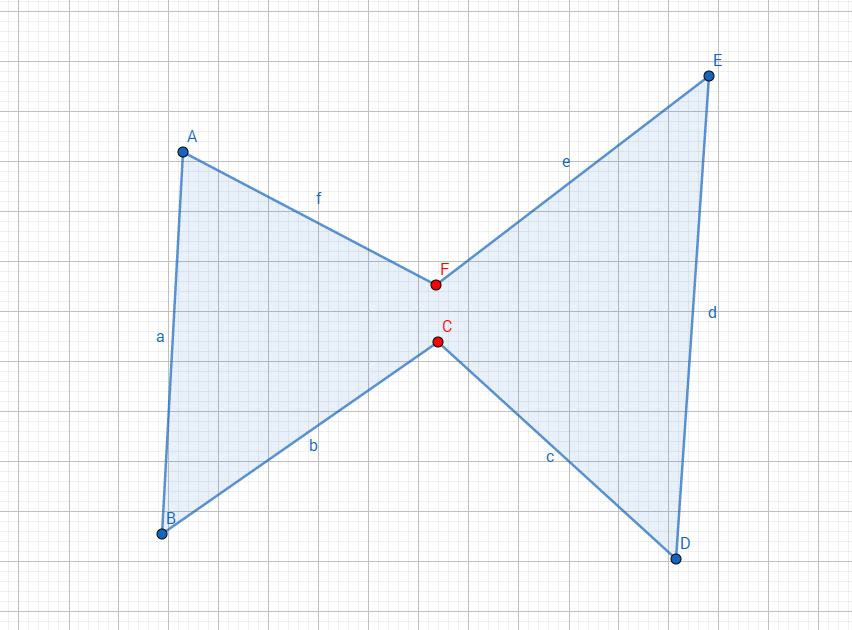
\includegraphics[width=0.95\textwidth]
        {figures/cut1.png}
        \caption{分割前的多边形}
    \end{minipage}
    \begin{minipage}{0.4\textwidth}
        \centering
        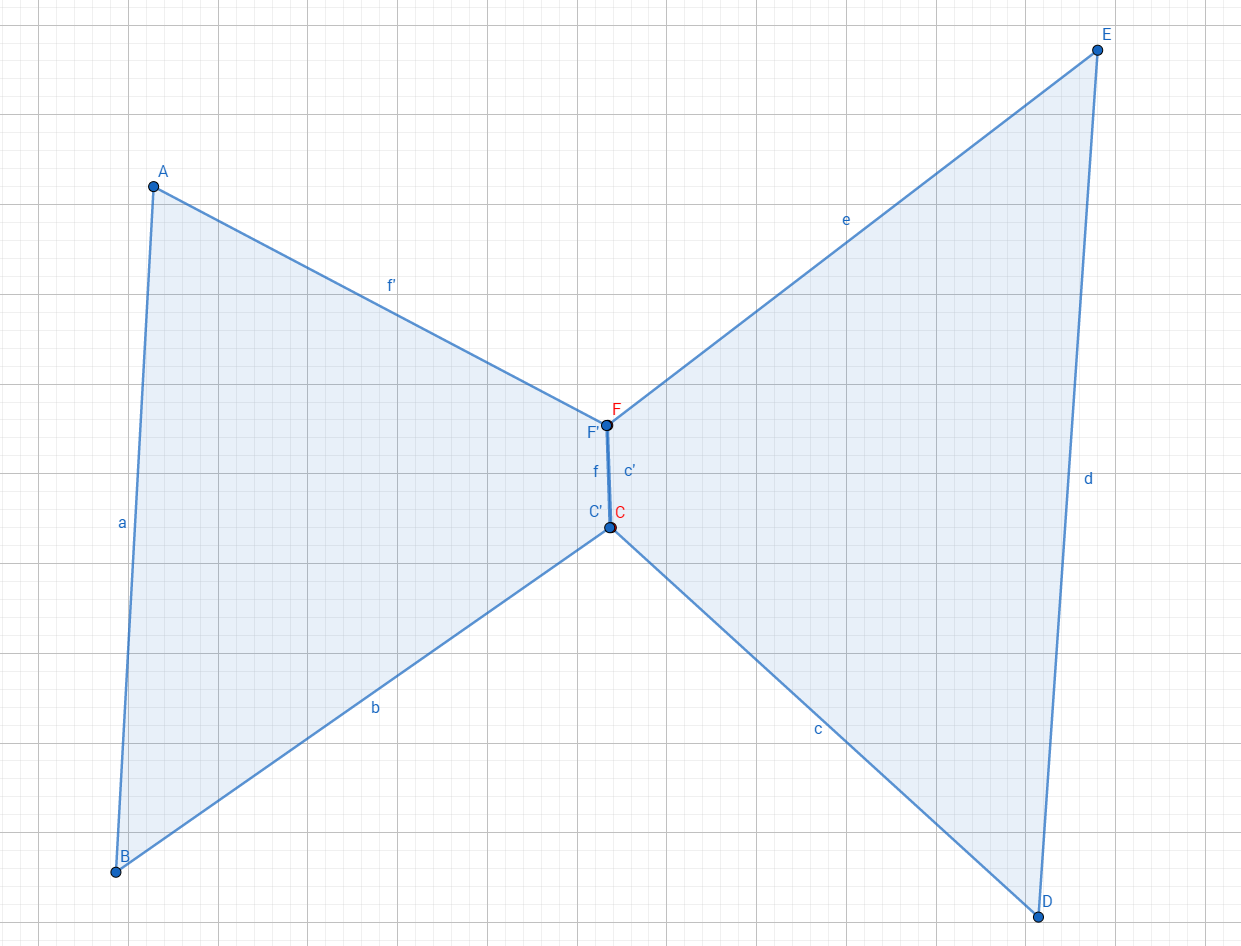
\includegraphics[width=0.95\textwidth]
        {figures/cut2.png}
        \caption{在待分割点的逆时针方向新增等位点}
    \end{minipage}
\end{figure}

以这种方案实现对多边形的分割时,可以巧妙的准确找到每个分割边所对应的顶点的真实位置。即使顶点被复制多次,初始指向顶点的指针指向了错误的多边形,也可以利用栈找到每个指针的正确位置。

完成上述流程后,原本的一个凹多边形将被分为数个部分,我们只需递归的对每个子多边形使用相同方式进行处理即可。

\begin{figure}[htp]
    \centering
    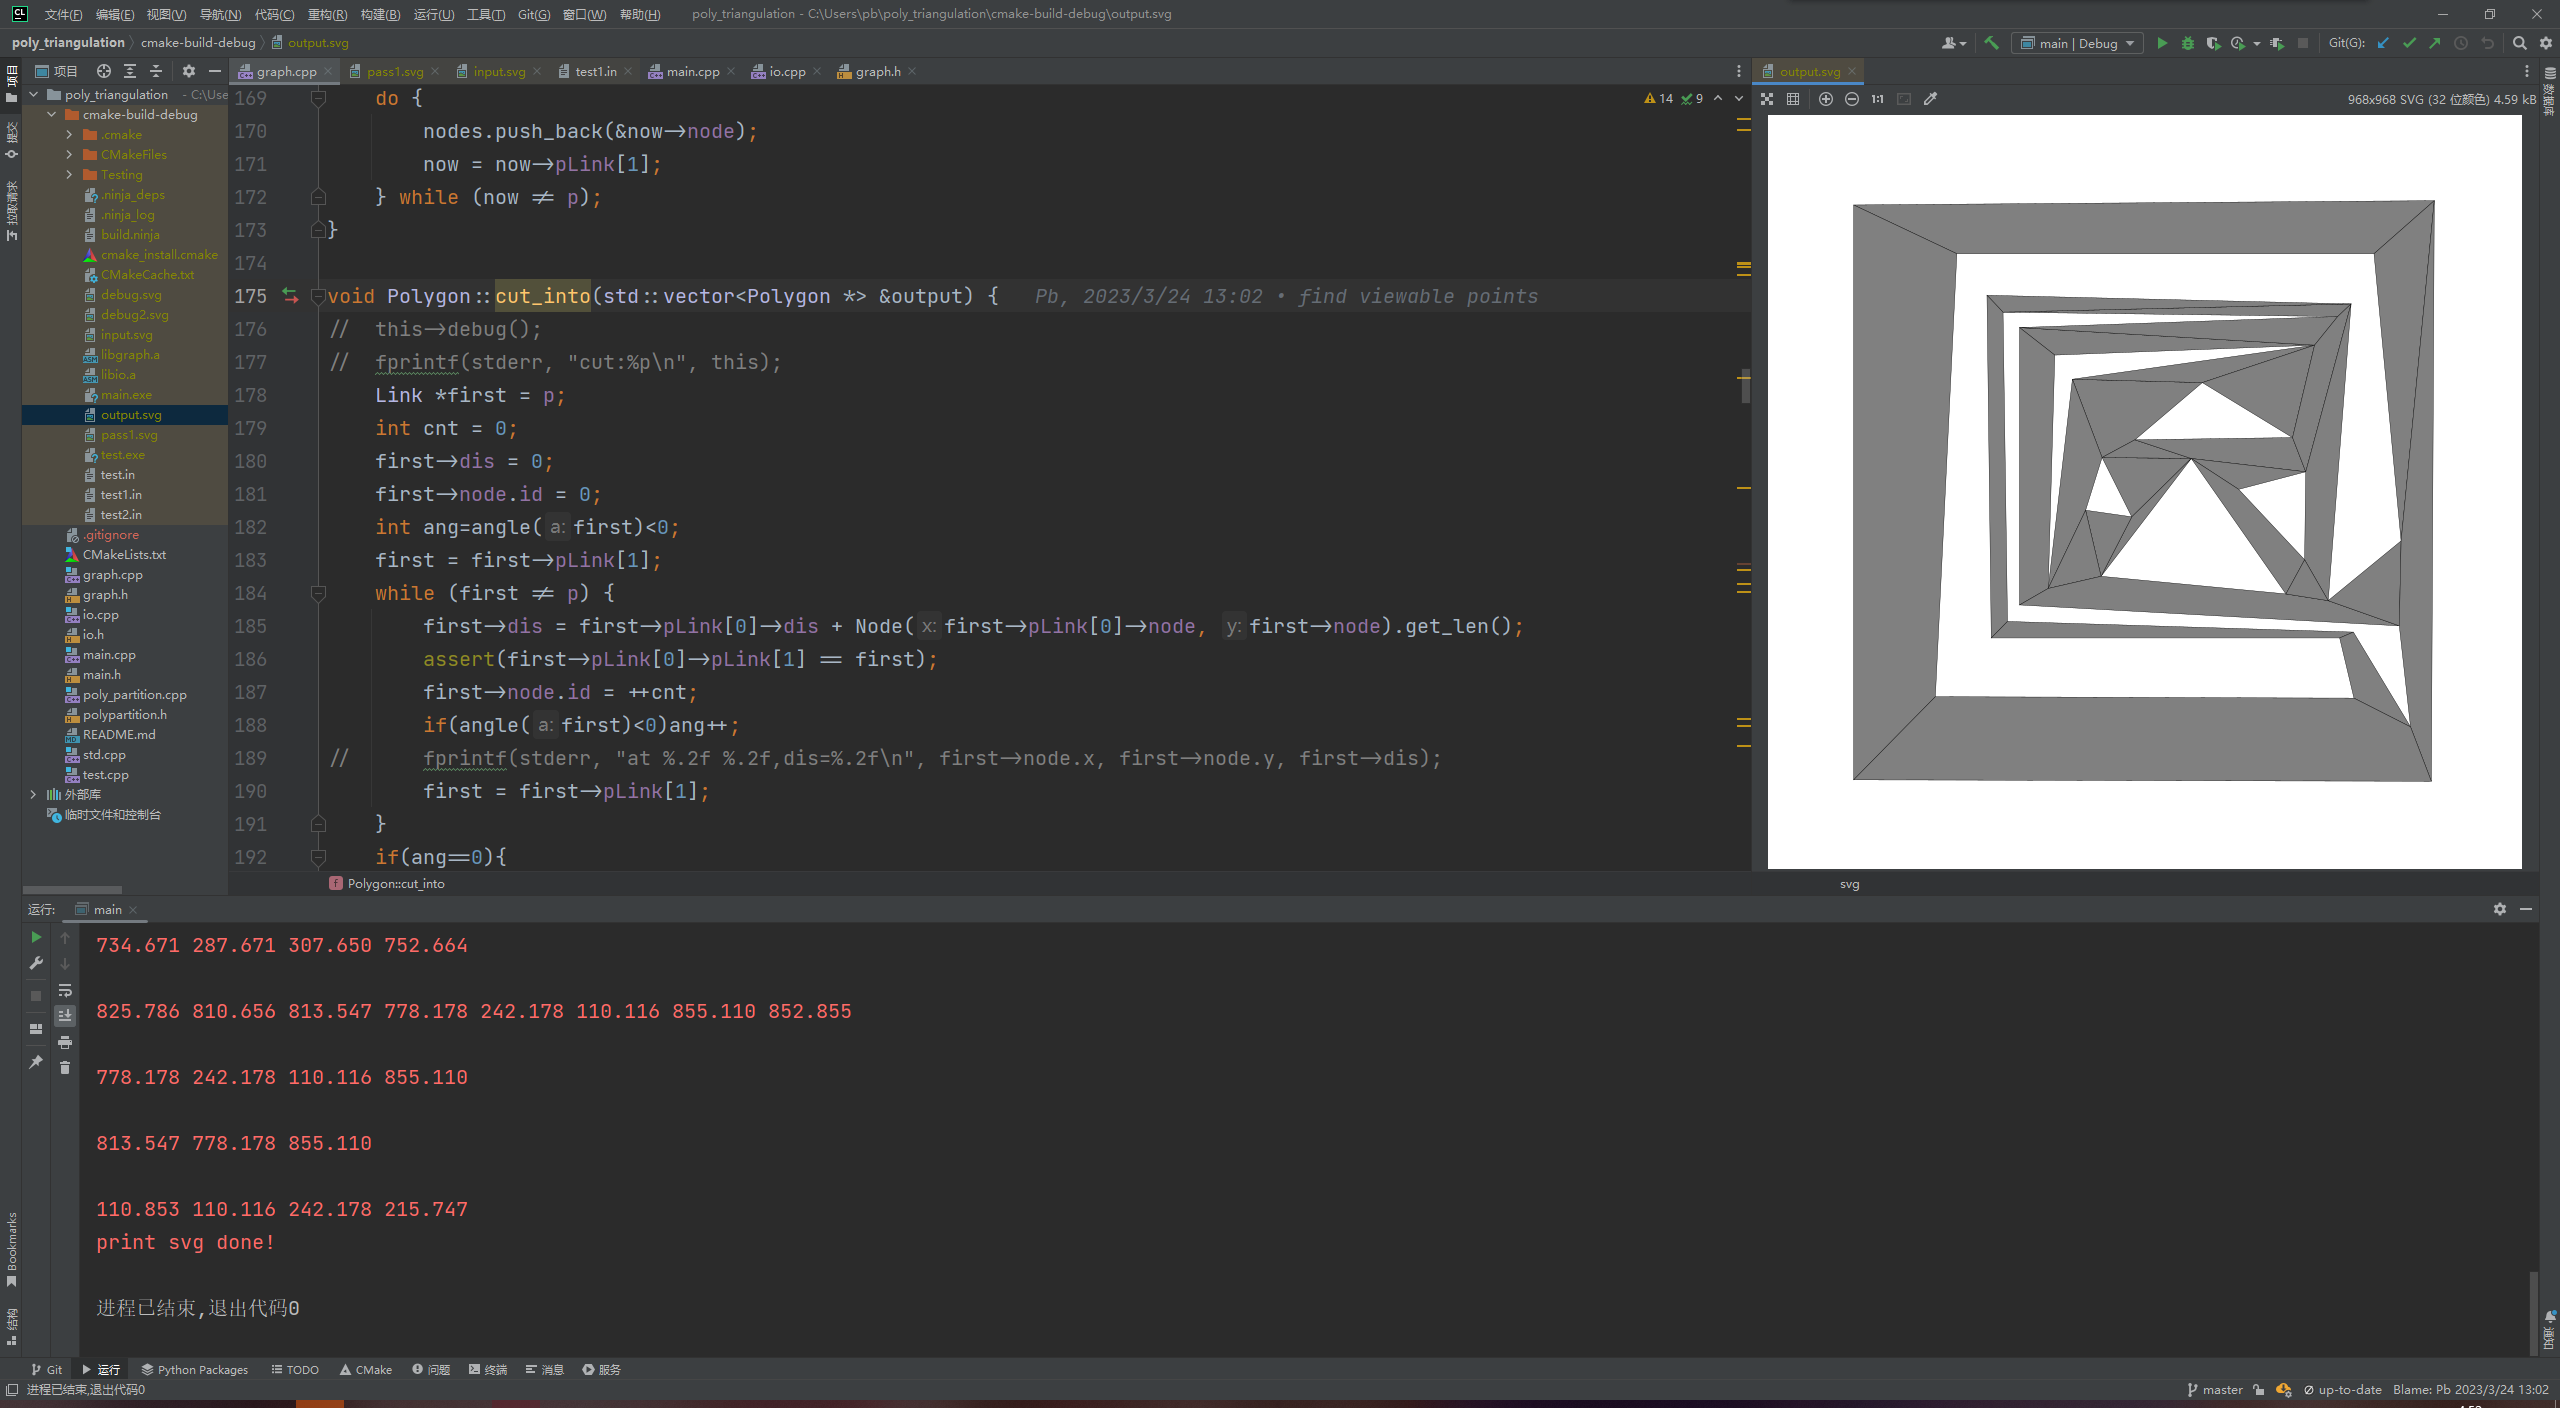
\includegraphics[width=0.9\textwidth]
    {figures/output.png}
    \caption{代码运行到此步的结果}
  \end{figure}

%待补充图片与详细解释
\section{一些其他的改进思路}
本算法可以较为有效的将凹多边形分割为数个凸多边形,但生成分割边时将会尽可能多的对原多边形进行分割,可能会在单个凹点处进行过多的切割,导致出现较小的锐角。对应图~\ref*{pass1}的情况,尽可能多的选择分割边时将会对一些评分较低不需要进行分割,但并未和已选边产生冲突的垃圾边也进行切割,导致产生大量的细长三角形。以下是一些改进本算法的思路。

\subsection{限制分割线数量}
在确定可行分割方案的过程中,默认采用了贪心算法,只要存在可行的分割方法就会加入结果中。因此可能会出现从一个凹顶点连线到凸多边形每个顶点进行分割的情况;而理想情况下本章算法的目标为用相对较少的线段将输入的凹多边形分割为数个凸多边形。因此,我们可以对分割线的数量进行限制。

在较为理想的情况下,每一条分割线可以消除1-2个凹点。也就是说,将一个凹多边形分割为数个凸多边形时,使用的分割线数目很可能少于凹顶点的数目。因此,我们可以限制每次选择分割方案的数目上限。

我们可以在算法的开始阶段记录当前多边形的凹顶点数目,并将其乘上一个修正量后作为分割线的最大数目。在依次检验分割方案是否与已选中部分冲突时,若已选中的分割线数目已经等于最大数目,则丢弃剩余的所有方案,只使用有限数量的分割线进行分割。由于被分割出的小多边形会用递归的方式再次经过本算法检验凹凸性并进行分割,算法的正确性不会受到影响。

正确的选择修正量可以在精确度与速度之中做出平衡。较大的修正量会产生更多的分割线,生成的小多边形将更不可能是需要重新执行本算法的凹多边形;而较小的修正量则能够获得较为优秀的划分结果,但会增加算法的运行时间。笔者认为,在实际计算中取0.5至1的修正量较为合适。

\subsection{禁止单个顶点进行多次切分}
在评估时,单个凹顶点可能有相似的数个较优秀候选切割边。这些切割边之间互不冲突,且评估价值相近。在筛选分割方案时,容易出现单个顶点选择数条同质切割边的情况。不仅会产生一些细长三角形,同时还影响算法效率。可以在切分时限制单个顶点最多被切分一次,跳过后续的相似切割边。
\subsection{动态调整启发函数}
在启发式函数中,采用的评估方案通过计算边长与切下的小多边形周长比值作为基础评分,以顶点凹凸性和最小角度数作为修正值。但在完成了一次切割后,后续的待选切割边两端的多边形周长将会发生变化,实际评估值将会改变,需要随时进行更新。考虑到实际评估值在分割过程中仅会下降不会上升,我们可以利用大根堆存储所有的切割方案,并在取新方案时对该方案进行更新并重新放入堆中,直到取出的方案已被更新过。

% \chapter{引用与链接}

% \section{脚注}
% 注释是对论文中特定名词或新名词的注解。注释可用页末注或篇末注的一种。选择页末注的应在注释与正文之间加细线分隔,线宽度为1磅,线的长度不应超过纸张的三分之一宽度。同一页类列出多个注释的,应根据注释的先后顺序编排序号。字体为宋体5号,注释序号以“\circled{1}、\circled{2}”等数字形式标示在被注释词条的右上角。页末或篇末注释条目的序号应按照“\circled{1}、\circled{2}”等数字形式与被注释词条保持一致。示例:这里有个注释\footnote{我是解释注释的}。

% \section{引用文中小节}\label{sec:ref}
% 如引用小节~\ref{sec:ref}

% \section{引用参考文献}
% 这是一个参考文献引用的范例

% 还可以采用上标的引用方式

% 引用多个文献

% 文献引用需要配合BibTeX使用,很多工具可以直接生成BibTeX文件(EndNote, NoteExpress, 百度学术,谷歌学术),此处不作介绍。

% \section{链接相关}
% 模板使用了hyperref处理相关链接,使用\verb|href|可以生成超链接,链接周围的方框在打印时不会出现。可以在cls文件中修改相应的hypersetup项来关闭方框:\verb|\hypersetup{hidelinks}|。如果需要输出网址,可以使用\verb|url|包,示例:\url{https://github.com}。